\documentclass[tikz,border=10pt]{standalone}
\usepackage{mathrsfs}
\usetikzlibrary{decorations.pathmorphing}
    % this is for graphics. e.g. rectangle on title page
\usetikzlibrary{3d,perspective}
\usetikzlibrary{backgrounds}
\usetikzlibrary{arrows,shapes,positioning,shadows,trees,mindmap}
\usetikzlibrary{tikzmark}
\usetikzlibrary{calc,math}

\usepackage{tikz-3dplot}
\usepackage{pgfplots}
\pgfplotsset{compat = newest}
%\usepgfplotslibrary{colormaps}
\usepgflibrary{shapes.geometric}

\usepackage[edges]{forest}
\usetikzlibrary{arrows.meta}
\colorlet{linecol}{black!75}
\usepackage{xkcdcolors} % xkcd colors

\usetikzlibrary{patterns}
\tikzset{>={Stealth[inset=0pt,angle=20:10pt]}}


\tikzset{zigzag/.style={decorate,decoration=zigzag}}


\begin{document}
    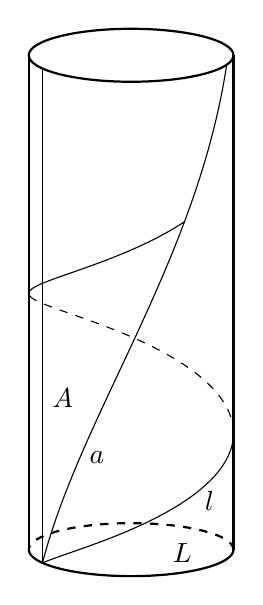
\begin{tikzpicture}[3d view={0}{15},scale=1.3]
        \def\h{5}
    \def\f{-150}
    \def\v{0.45}
    \draw[thick] (0,0,\h) circle(1);
    \draw[thick] (1,0,0) arc(0:-180:1);
    \draw[thick,dashed] (1,0,0) arc(0:180:1);
    \draw[thick] (1,0,0)--(1,0,\h);
    \draw[thick] (-1,0,0)--(-1,0,\h);
    \draw ({cos(\f)},{sin(\f)},0)--({cos(\f)},{sin(\f)},\h);
    \draw[domain=0:180*\h/pi*\v,samples=200] plot({cos(\f+\x)},{sin(\f+\x)},{\x*pi/180/\v});
    \draw[domain=0:-\f,samples=200] plot({cos(\f+\x)},{sin(\f+\x)},{\x*pi*\v/180});
    \draw[dashed,domain=-\f:180-\f,samples=200] plot({cos(\f+\x)},{sin(\f+\x)},{\x*pi*\v/180});
    \draw[domain=180-\f:360/(1-\v*\v),samples=200] plot({cos(\f+\x)},{sin(\f+\x)},{\x*pi*\v/180});
    \node at ({cos(\f)},{sin(\f)},\h/3) [right]{$A$};
    \node at ({cos(\f+30)},{sin(\f+30)},{30*pi/\v/180}) [right]{$a$};
    \node at ({cos(-60)},{sin(-60)},0)[above]{$L$};
    \node at ({cos(\f+110)},{sin(\f+110)},{110*pi*\v/180}) [below]{$l$};
    \end{tikzpicture} 
\end{document}